% EECS 182 final project report -- draft.
% Compile: pdflatex main && bibtex main && pdflatex main && pdflatex main (or upload report/ + figures/ to Overleaf)
% Figures are read from ../figures/ (regenerate with: .venv/bin/python analysis/plots.py).
% For a venue submission, swap the preamble for the venue's style file (e.g. neurips_2026.sty); the body is style-agnostic.
\documentclass[11pt]{article}

\usepackage[margin=1in]{geometry}
\usepackage[T1]{fontenc}
\usepackage{lmodern}
\usepackage{microtype}
\usepackage{amsmath,amssymb,amsthm}
\usepackage{booktabs}
\usepackage{multirow}
\usepackage{graphicx}
\usepackage{subcaption}
\usepackage{xcolor}
\usepackage[numbers,sort&compress]{natbib}
\usepackage[colorlinks=true,linkcolor=blue!50!black,citecolor=blue!50!black,urlcolor=blue!50!black]{hyperref}
\usepackage[capitalise,noabbrev]{cleveref}

\graphicspath{{../figures/}}

\newcommand{\todo}[1]{\textcolor{red}{[TODO: #1]}}
\newcommand{\Lhet}{\Delta L_{\mathrm{het}}}
\newcommand{\E}{\mathbb{E}}
\newcommand{\R}{\mathbb{R}}

\title{Muon Workers Drift Further:\\ Data Heterogeneity in Low-Communication Training with Muon}

\author{
  Abhay Paidipalli\thanks{Equal contribution.} \quad Ethan Liu\footnotemark[1] \quad
  Logan Wall\footnotemark[1] \quad Prabhnoor Rai\footnotemark[1] \\[2pt]
  University of California, Berkeley \\
  \texttt{\{abhayp, ethanl\_, loganwall, prabhnoorrai\}@berkeley.edu}
}

\date{}

\begin{document}
\maketitle

% ======================================================================================================
\begin{abstract}
DiLoCo trains a language model on several workers that each take many local optimizer steps between synchronizations, and MuLoCo shows that replacing DiLoCo's inner AdamW with Muon improves this regime. Both results, however, are obtained with every worker sampling the same data distribution. Federated-learning theory predicts that when workers see different data, local steps drift toward each worker's own optimum, and recent analyses of orthogonalized local updates suggest Muon may be especially exposed. To test this hypothesis directly, we pretrain 51M-parameter GPT models from scratch on four text domains (ArXiv, GitHub, StackExchange, Wikipedia) with four workers, varying a deterministic skew from IID to one-domain-per-worker while holding the global data mixture fixed, and compare DiLoCo, MuLoCo, their plain-averaging (FedAvg) counterparts, and single-worker baselines. Muon keeps the lower loss at every heterogeneity level, but its heterogeneity penalty is larger: $+0.135 \pm 0.009$ vs.\ $+0.101 \pm 0.006$ nats at full skew, so MuLoCo's advantage shrinks by a third and its gap to its own single-worker baseline matches DiLoCo's. Outer Nesterov momentum, the component that distinguishes DiLoCo from FedAvg, slightly reduces AdamW's penalty but gives Muon no benefit. Standard parameter-space drift diagnostics (norm retention, interference gap, alignment with a data-parallel reference) rank the methods the wrong way; a function-space measure, how much each worker's local model specializes to its home domain within a round, does not, and is $1.7\times$ larger for Muon workers. Code, logs, and checkpoints are public.\footnote{\url{https://github.com/abhay1105/muloco-data-heterogeneity}}\footnote{\url{https://huggingface.co/paidvenk/muloco-data-heterogeneity}}
\end{abstract}

% ======================================================================================================
\section{Introduction}

Training large language models normally requires tightly coupled accelerators that exchange gradients at every step. Low-communication methods relax this: in DiLoCo~\cite{douillard2023diloco}, each of $K$ workers runs $H$ inner optimizer steps (AdamW) from a shared model, the workers' parameter changes (\emph{pseudo-gradients}) are averaged, and an outer optimizer (Nesterov momentum) applies the average. Communication drops by a factor of $H$ with little loss in quality, and the method has since been scaled and extended~\cite{jaghouar2024opendiloco,douillard2025streaming,charles2025scaling}. MuLoCo~\cite{therien2025muloco} replaced the inner AdamW with Muon~\cite{jordan2024muon}, an optimizer that orthogonalizes each weight matrix's momentum, and found that it lowers loss and makes pseudo-gradients more compressible and better aligned with the data-parallel update.

These results share one assumption: every worker samples from the same distribution. In settings that motivate low-communication training in the first place (training across data centers, organizations, or data sources that
cannot be pooled), workers' data are often different. Federated learning (FL) has studied this regime for years. Its central finding is \emph{client drift}: with heterogeneous data, local steps move each worker toward its own optimum, and averaging the results converges to a biased point~\cite{zhao2018noniid,karimireddy2020scaffold,wang2020fednova}. Two recent analyses make a sharper prediction for Muon. \citet{takezawa2026fedmuon} show that naively running LMO-based optimizers such as Muon locally does not converge under heterogeneity, and that server-side momentum does not fix it. \citet{liu2025fedmuon}, by contrast, find local Muon outperforming local AdamW on non-IID image classification. Whether MuLoCo's advantage survives heterogeneous data in language-model pretraining, and whether DiLoCo's outer momentum protects it, is open.

\paragraph{Our contributions.} We run a controlled study with four workers that each favor one of four text domains. A single skew parameter $p$ interpolates from IID ($p=0.25$) to one domain per worker ($p=1$) while the \emph{global} data mixture, and hence the objective and the single-worker baselines, stays fixed (\cref{sec:setup}). We ask two questions, each stated as competing predictions before any experiment runs (\cref{sec:hypotheses}):
\begin{itemize}
  \item \textbf{H1.} Does MuLoCo's heterogeneity penalty grow faster than DiLoCo's (the FL prediction), or does its better conditioning keep it equal or smaller (the MuLoCo prediction)?
  \item \textbf{H2.} Does outer Nesterov momentum reduce the penalty relative to plain averaging (FedAvg), and more so for Muon?
\end{itemize}

\paragraph{Key Findings}
\begin{enumerate}
  \item MuLoCo has the lower validation loss at every skew level, but its heterogeneity penalty is larger at every level and grows faster with skew (slope $0.174$ vs.\ $0.129$ nats per unit total-variation distance). At full skew the excess is $+0.034 \pm 0.009$ nats, consistent in sign on all seeds and above our pre-registered threshold. MuLoCo's lead over DiLoCo shrinks from $0.105$ to $0.071$ nats, and both methods end ${\approx}13.5\%$ above their own single-worker baselines (\cref{sec:h1}).
  \item Outer momentum reduces AdamW's penalty only slightly ($0.010$ nats) and does not reduce Muon's at all ($-0.009$); FedAvg-Muon and MuLoCo are indistinguishable at full skew. H2's predicted ordering is reversed (\cref{sec:h2}).
  \item Parameter-space drift diagnostics (norm retention, interference gap, cosine to a data-parallel reference step) say MuLoCo's pseudo-gradients are \emph{better} aligned and degrade \emph{less} with skew, which contradicts its larger loss penalty. A function-space diagnostic, how far each worker's local model moves toward its home domain within one round, is $1.7\times$ larger for Muon-based workers and orders all four methods the same way as their penalties (\cref{sec:mechanism}).
\end{enumerate}

% ======================================================================================================
\section{Background and related work}\label{sec:related}

\paragraph{Local SGD, federated averaging, and client drift.} Periodically averaged local training goes back to local SGD and federated averaging (FedAvg)~\cite{mcmahan2017fedavg,stich2019local,lin2020dont}. With heterogeneous data, local updates are biased toward each client's objective; this \emph{client drift} slows or biases convergence~\cite{zhao2018noniid,kairouz2021advances}. Remedies include proximal terms (FedProx~\cite{li2020fedprox}), control variates (SCAFFOLD~\cite{karimireddy2020scaffold}), normalized averaging
(FedNova~\cite{wang2020fednova}), and server-side optimizers including momentum and adaptive methods~\cite{hsu2019measuring,reddi2021adaptive}. Heterogeneity is usually simulated with Dirichlet label partitions~\cite{hsu2019measuring}; we instead use a
deterministic domain skew that keeps the global mixture fixed (\cref{sec:data}).

\paragraph{DiLoCo and outer optimizers.} DiLoCo~\cite{douillard2023diloco} is FedAvg with AdamW inner steps and an outer Nesterov optimizer applied to the
averaged pseudo-gradient. Its authors found plain outer averaging clearly worse than Nesterov even on IID data, and reported robustness to non-IID shards made by clustering C4, starting from a pretrained model. Follow-ups scale DiLoCo~\cite{jaghouar2024opendiloco,charles2025scaling} and reduce its communication further~\cite{douillard2025streaming}; HeLoCo~\cite{alasif2026heloco} studies asynchronous DiLoCo under data and device heterogeneity and uses agreement with the outer momentum as a drift signal.

\paragraph{Muon and MuLoCo.} Muon~\cite{jordan2024muon} keeps a momentum buffer for each hidden weight matrix and replaces it with an approximation of
its nearest semi-orthogonal matrix (the polar factor, computed by a few Newton-Schulz iterations) before stepping. It can be viewed as steepest descent under a spectral norm, i.e.\ a linear-minimization-oracle (LMO)
method~\cite{bernstein2024oldoptimizer}, and scales to large LLM training when its update is rescaled to match AdamW's root-mean-square size~\cite{liu2025muonscalable}. MuLoCo~\cite{therien2025muloco} uses Muon as DiLoCo's inner optimizer and finds lower loss and better pseudo-gradient alignment than DiLoCo, on IID data only.

\paragraph{Muon under heterogeneity.}
\citet{takezawa2026fedmuon} prove that running an LMO-based method locally and averaging does not converge to a stationary point under heterogeneity, show server momentum does not remove the bias, and propose a SCAFFOLD-style
correction. \citet{liu2025fedmuon} report local Muon beating local AdamW on non-IID CIFAR with momentum aggregation and a local-global alignment term. Neither studies language-model pretraining or DiLoCo's outer optimizer; our work measures the effect in that setting with matched tuning and multiple seeds.

% ======================================================================================================
\section{Setup}\label{sec:setup}

\subsection{Methods}
Let $\theta^{(r)}$ be the shared (\emph{outer}) parameters at round $r$. Each worker $k \in \{1,\dots,K\}$ copies $\theta^{(r)}$, takes $H$ steps of an inner optimizer on its own data stream, and returns $\theta_k^{(r)}$. The pseudo-gradient is
\begin{equation}
  \Delta_k = \theta^{(r)} - \theta_k^{(r)}, \qquad \bar\Delta = \frac{1}{K}\sum_{k=1}^K \Delta_k,
\end{equation}
and the outer optimizer treats $\bar\Delta$ as a gradient. With Nesterov momentum (PyTorch convention),
\begin{equation}
  m \leftarrow \mu m + \bar\Delta, \qquad \theta^{(r+1)} = \theta^{(r)} - \eta_{\mathrm{out}}\,(\bar\Delta + \mu m).
\end{equation}
FedAvg is the special case $\eta_{\mathrm{out}} = 1$, $\mu = 0$, i.e.\ $\theta^{(r+1)} = \frac1K\sum_k \theta_k^{(r)}$.
We compare six methods, crossing the inner optimizer with the outer scheme:

\begin{center}
\begin{tabular}{lll}
  \toprule
  & Inner AdamW & Inner Muon \\
  \midrule
  Outer Nesterov & DiLoCo~\cite{douillard2023diloco} & MuLoCo~\cite{therien2025muloco} \\
  Outer plain averaging & FedAvg-AdamW & FedAvg-Muon \\
  Single worker (data-parallel) & DP-AdamW & DP-Muon \\
  \bottomrule
\end{tabular}
\end{center}

Muon is applied to every 2D weight matrix inside the transformer blocks; the tied embedding/output matrix and the normalization gains use AdamW, identically in DP-Muon, MuLoCo and FedAvg-Muon. Muon's update for a matrix
$W \in \R^{m\times n}$ with momentum buffer $B$ and gradient $G$ is
$W \leftarrow W - \eta \cdot 0.2\sqrt{\max(m,n)}\cdot \mathrm{NS}_5(G + \beta B)$, where $\mathrm{NS}_5$ is five Newton-Schulz iterations approximating the polar factor and the $0.2\sqrt{\max(m,n)}$ factor puts Muon learning rates on AdamW's scale~\cite{liu2025muonscalable}. Each worker keeps its own inner optimizer state across rounds; states are never averaged or reset, following DiLoCo.

\subsection{Data and heterogeneity}\label{sec:data}
We use four domains: ArXiv, GitHub, and StackExchange from SlimPajama-6B (a subsample of SlimPajama~\cite{cerebras2023slimpajama}) and English Wikipedia (20231101 dump~\cite{wikimedia2023wikipedia}), tokenized with the GPT-2 tokenizer~\cite{radford2019gpt2}. Each domain contributes exactly $122.88$M training tokens, $1.02$M validation tokens, and a separate $2.1$M-token probe pool. Dataset revisions are pinned and the processed data are identified by a content hash.

Worker $k$ has home domain $k$. A skew parameter $p \in \{0.25, 0.5, 0.75, 1\}$ sets worker $k$'s mixture to fraction $p$ from its home domain and $(1-p)/3$ from each other domain. Each domain's training tokens are cut into disjoint slices in these proportions, so every column of the allocation matrix sums to one: the \emph{global} mixture is uniform for every $p$, every method trains on the same token multiset, and no token is seen twice. We report heterogeneity as the total-variation distance between a worker's mixture and the global mixture, $h = p - 0.25 \in \{0, 0.25, 0.5, 0.75\}$. Unlike Dirichlet partitions, this keeps the objective identical across
heterogeneity levels, so the single-worker baselines are shared and differences in loss are attributable to how the data is distributed rather than what data is used.

\subsection{Model and training}
The model is a decoder-only transformer with 8 layers, width 512, 8 heads, RoPE~\cite{su2024roformer}, RMSNorm~\cite{zhang2019rmsnorm}, QK-normalization~\cite{henry2020qknorm}, GELU MLPs, no biases and a tied embedding (50.9M parameters, 25.2M outside the embedding). Every run trains for 7{,}500 steps at 65{,}536 tokens per step (${\approx}0.49$B tokens, about 19.5 tokens per non-embedding parameter). Local methods use $K=4$ workers with 16 sequences each per step and synchronize every $H=30$ steps (250 rounds); DP baselines take 64 sequences per step on the shuffled union of the same data. Learning rates warm up linearly for 250 steps and follow a cosine decay to $0.1\times$ peak; weight decay is zero; gradients are clipped to norm 1 per worker. Workers are simulated sequentially on one GPU, which changes wall-clock time but not the computation.

\subsection{Tuning protocol}
All hyperparameters were tuned on IID data only and frozen before any heterogeneous run. (1)~DP learning-rate sweeps at full length chose AdamW $1.5\times10^{-3}$ and Muon $1.2\times10^{-2}$ (with AdamW $1.5\times10^{-3}$ for the non-Muon parameters); these runs double as the seed-0 DP baselines. (2)~A half-length sweep over $\eta_{\mathrm{out}} \in \{0.5, 0.8, 1.0\}$ and $\mu \in \{0, 0.3, 0.6, 0.9\}$ chose $(0.8, 0.6)$ for both DiLoCo and
MuLoCo. (3)~A check of the inner learning rate at that outer setting lowered DiLoCo's inner rate to $7.5\times10^{-4}$ and left MuLoCo's unchanged (its loss was flat within $0.002$ over a $4\times$ range). FedAvg arms reuse the inner rates of their Nesterov counterparts. Full sweep results are in \cref{app:tuning}.

\subsection{Metrics, hypotheses and decision rules}\label{sec:hypotheses}
The primary metric is the domain-balanced validation loss $L$ (mean of the four per-domain losses) of the outer model after training, on the full 1M-token validation set per domain. The \emph{heterogeneity penalty} of method $m$ is $\Lhet(m, p) = L(m, p) - L(m, 0.25)$, computed per seed (seeds fix initialization and data order and are shared across methods, so differences are paired) and then averaged. We also report the gap to the same optimizer's DP baseline, $G_{\mathrm{DP}} = L/L_{\mathrm{DP}} - 1$.

\textbf{H1} contrasts two predictions: \emph{H1-FL}, $\Lhet$ grows faster with $h$ for MuLoCo; \emph{H1-MuLoCo}, MuLoCo's penalty is equal or smaller. \emph{Decision rule (fixed in advance):} at $h=0.75$, compare the per-seed
differences $\Lhet(\mathrm{MuLoCo}) - \Lhet(\mathrm{DiLoCo})$; a direction is declared only if all differences share a sign and their mean exceeds twice the across-seed standard deviation of the IID runs.

\textbf{H2} predicts that outer momentum rescues Muon more than AdamW. For inner optimizer $i$, the rescue is the difference-in-differences
\begin{equation}
  R_i = \big[L(\text{FedAvg}_i, 1) - L(\text{FedAvg}_i, 0.25)\big] - \big[L(\text{Nest}_i, 1) - L(\text{Nest}_i, 0.25)\big],
\end{equation}
and H2 predicts $R_{\mathrm{Muon}} > R_{\mathrm{AdamW}} > 0$ with a nonzero residual penalty under Nesterov.

All production conditions use three seeds: 24 runs for DiLoCo/MuLoCo $\times$ 4 skews, 12 for FedAvg $\times$ $\{0.25, 1\}$, and 6 DP baselines, 42 runs in total, none of which diverged. Error bars are $\pm$ one sample standard deviation over seeds. The production runs used about 18 A100-hours (24 GPU-hours including tuning).

\subsection{Drift diagnostics}\label{sec:diagnostics}
On the Muon-managed hidden matrices (identical tensors in all methods) we log, every round: the \emph{norm retention} $\rho_F = \lVert\bar\Delta\rVert_F / \frac1K\sum_k\lVert\Delta_k\rVert_F$ (1 for identical workers, $1/\sqrt{K}=0.5$ for orthogonal equal-norm workers); the mean pairwise cosine between $\Delta_k$'s; and, for Nesterov runs, the cosine
between $\bar\Delta$ and the outer momentum. Every 300 steps we compute the nuclear-norm retention $\rho_*$ and the normalized interference gap of \citet{therien2025muloco} over the top 5\% of singular values. At 25/50/75\% of training we also compute (i) the cosine between $\bar\Delta$ and a reference pseudo-gradient from $H$ data-parallel steps on the
uniform probe pool from the same starting point and averaged optimizer state, and (ii) a $4\times4$ \emph{specialization matrix} of each worker's local model evaluated on each domain before averaging.

% ======================================================================================================
\section{Results}\label{sec:results}

\begin{figure}[t]
  \centering
  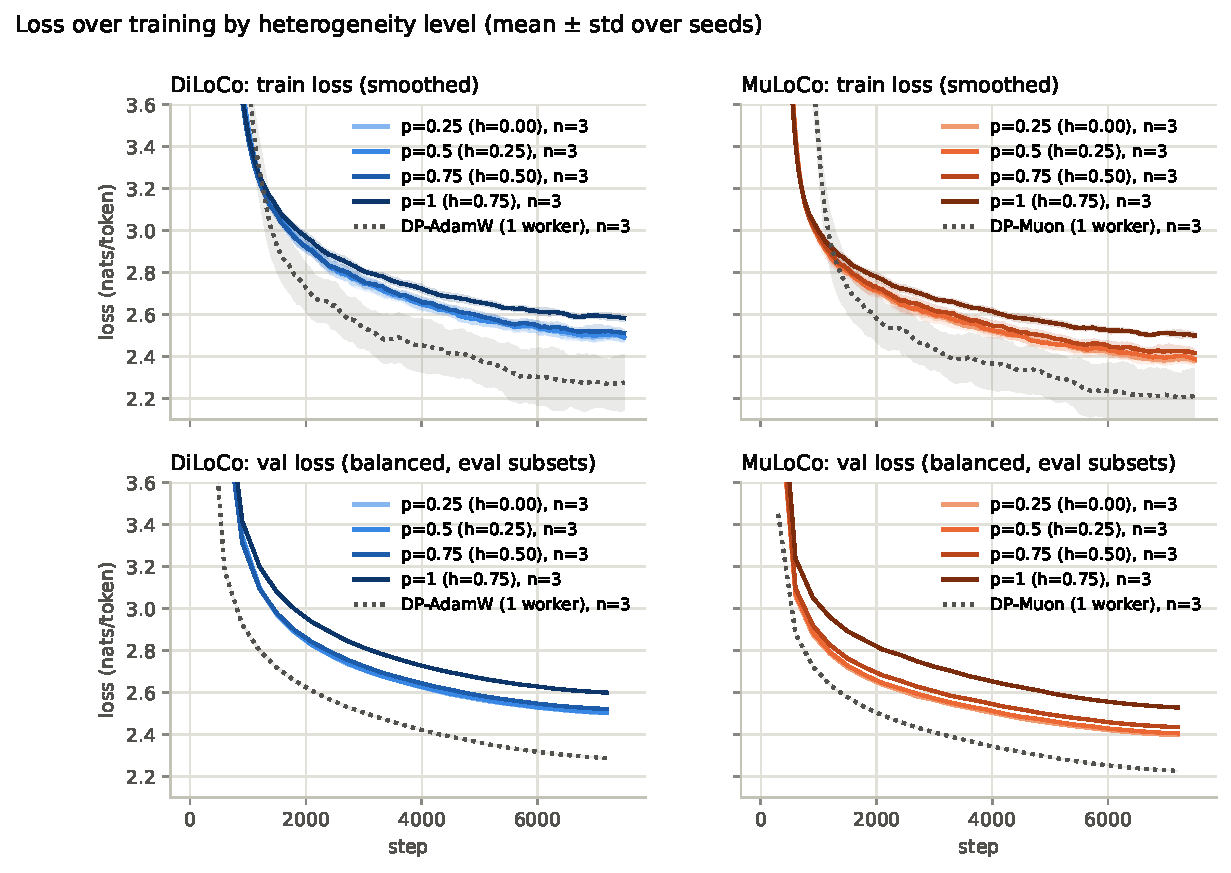
\includegraphics[width=\linewidth]{fig1_loss_curves.pdf}
  \caption{Training (top, smoothed) and validation (bottom) loss of DiLoCo (left) and MuLoCo (right) at each skew level, with the same optimizer's single-worker DP baseline dotted. Bands are $\pm 1$ std over 3 seeds. Validation curves use fixed 256K-token subsets per domain; final numbers in the tables use the full 1M-token sets, which read ${\approx}0.02$ higher. The penalty from skew appears early and persists to the end of training.}
  \label{fig:curves}
\end{figure}

\subsection{IID baseline}
On IID data MuLoCo reaches $2.420 \pm 0.006$ and DiLoCo $2.525 \pm 0.006$ (\cref{tab:final}), reproducing MuLoCo's advantage~\cite{therien2025muloco} at our scale. Both remain above their single-worker baselines (DP-Muon $2.251$, DP-AdamW $2.312$), by $7.5\%$ and $9.2\%$ respectively, and FedAvg is worse than Nesterov for both inner optimizers. Learning curves (\cref{fig:curves}) are smooth and none of the 42 production runs diverged.

\begin{table}[t]
  \centering
  \caption{Final domain-balanced validation loss (nats/token), mean $\pm$ std over 3 seeds. Lower is better. DP baselines train on the same data with one worker and do not depend on $p$.}
  \label{tab:final}
  \small
  \begin{tabular}{lcccc}
    \toprule
    Method & $p=0.25$ ($h=0$, IID) & $p=0.5$ ($h=0.25$) & $p=0.75$ ($h=0.5$) & $p=1$ ($h=0.75$) \\
    \midrule
    DiLoCo       & $2.5245 \pm 0.0064$ & $2.5263 \pm 0.0090$ & $2.5442 \pm 0.0026$ & $2.6259 \pm 0.0057$ \\
    MuLoCo       & $\mathbf{2.4196 \pm 0.0062}$ & $\mathbf{2.4282 \pm 0.0037}$ & $\mathbf{2.4568 \pm 0.0030}$ & $2.5548 \pm 0.0031$ \\
    FedAvg-AdamW & $2.5806 \pm 0.0042$ & -- & -- & $2.6915 \pm 0.0034$ \\
    FedAvg-Muon  & $2.4264 \pm 0.0051$ & -- & -- & $\mathbf{2.5528 \pm 0.0038}$ \\
    \midrule
    DP-AdamW (1 worker) & \multicolumn{4}{c}{$2.3116 \pm 0.0032$} \\
    DP-Muon (1 worker)  & \multicolumn{4}{c}{$2.2507 \pm 0.0017$} \\
    \bottomrule
  \end{tabular}
\end{table}

\subsection{H1: Muon pays a larger heterogeneity penalty}\label{sec:h1}

\begin{figure}[t]
  \centering
  \begin{subfigure}{0.49\linewidth}
    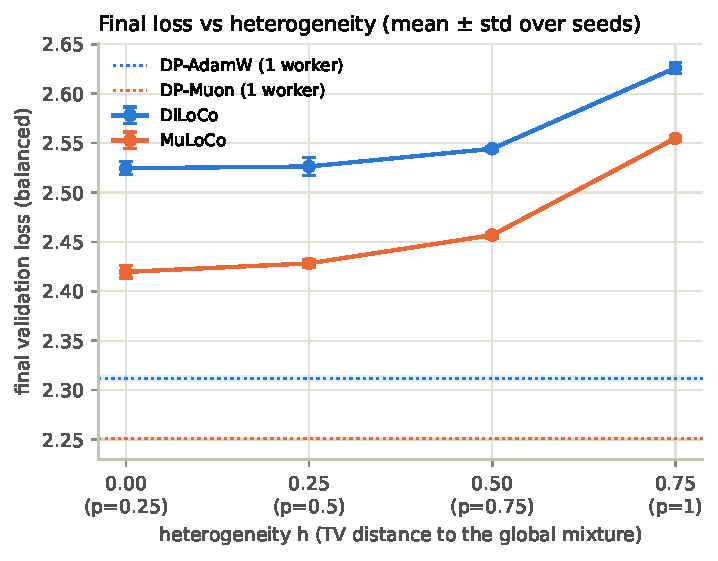
\includegraphics[width=\linewidth]{fig2_final_vs_h.pdf}
    \caption{Final loss vs.\ heterogeneity.}
    \label{fig:final_vs_h}
  \end{subfigure}\hfill
  \begin{subfigure}{0.49\linewidth}
    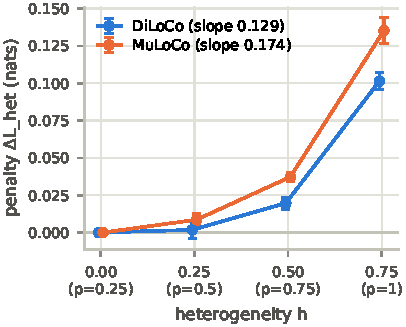
\includegraphics[width=\linewidth]{fig3_delta_het.pdf}
    \caption{Heterogeneity penalty $\Lhet$ (paired by seed).}
    \label{fig:delta_het}
  \end{subfigure}
  \caption{(a) MuLoCo is better than DiLoCo at every skew, but the gap narrows; dotted lines and bands are the DP
  baselines. (b) The penalty is convex in $h$ and larger for MuLoCo at every $h>0$. Error bars: $\pm1$ std over 3 seeds.}
  \label{fig:h1}
\end{figure}

Both methods lose little at mild skew and much more at full skew: the penalty is convex in $h$ (\cref{fig:delta_het}, \cref{tab:h1}). At every $h>0$, MuLoCo's penalty is larger, and the per-seed differences are positive on all three seeds at every level. At $h = 0.75$, the difference is $+0.034 \pm 0.009$ nats (per seed $+0.041, +0.037, +0.024$), well above the pre-registered threshold of $2 \times 0.0064 = 0.013$; at $h = 0.5$, it is $+0.018 \pm 0.002$, also above threshold; at $h = 0.25$, it is $+0.007 \pm 0.003$, below threshold. By our decision rule, \textbf{H1-FL is supported:
Muon's heterogeneity penalty grows faster than AdamW's.} A least-squares fit of $\Lhet$ against $h$ gives slopes of $0.174$ (MuLoCo) and $0.129$ (DiLoCo) nats per unit $h$.

This does not overturn MuLoCo's advantage in absolute terms: it remains ahead at full skew by $0.071 \pm 0.007$ nats, down from $0.105 \pm 0.003$ at IID. Relative to each optimizer's own DP baseline, however, the advantage disappears: $G_{\mathrm{DP}}$ rises from $7.5\%$ to $13.5\%$ for MuLoCo and from $9.2\%$ to $13.6\%$ for DiLoCo.

\begin{table}[t]
  \centering
  \caption{H1. Heterogeneity penalty $\Lhet = L(p) - L(0.25)$, paired by seed (mean $\pm$ std over 3 seeds), its least-squares slope against $h$, and the gap to the same optimizer's DP baseline.}
  \label{tab:h1}
  \small
  \begin{tabular}{lccccc}
    \toprule
    & $h=0.25$ & $h=0.5$ & $h=0.75$ & slope & $G_{\mathrm{DP}}$: IID $\to$ $h=0.75$ \\
    \midrule
    DiLoCo & $+0.0018 \pm 0.0057$ & $+0.0197 \pm 0.0040$ & $+0.1014 \pm 0.0059$ & $0.129$ & $9.2\% \to 13.6\%$ \\
    MuLoCo & $+0.0086 \pm 0.0040$ & $+0.0373 \pm 0.0032$ & $+0.1352 \pm 0.0086$ & $0.174$ & $7.5\% \to 13.5\%$ \\
    \midrule
    MuLoCo $-$ DiLoCo & $+0.0069 \pm 0.0030$ & $+0.0176 \pm 0.0015$ & $+0.0338 \pm 0.0086$ & & \\
    \bottomrule
  \end{tabular}
\end{table}

\paragraph{Where the penalty comes from.} Per domain (\cref{app:figures}, \cref{fig:heatmap}), Wikipedia, the domain least like the other three, carries most of the penalty: going from IID to full skew adds $+0.30$ (DiLoCo) and $+0.36$ (MuLoCo) nats on Wikipedia versus $+0.03$ to $+0.07$ elsewhere. MuLoCo's \emph{excess} penalty, however, appears on every domain (ArXiv $+0.061$ vs.\ $+0.036$; GitHub $+0.049$ vs.\ $+0.028$; StackExchange $+0.073$ vs.\ $+0.045$; Wikipedia $+0.358$ vs.\ $+0.297$), so it is not an artifact of one outlier domain.

\subsection{H2: outer momentum does not rescue Muon}\label{sec:h2}

\begin{figure}[t]
  \centering
  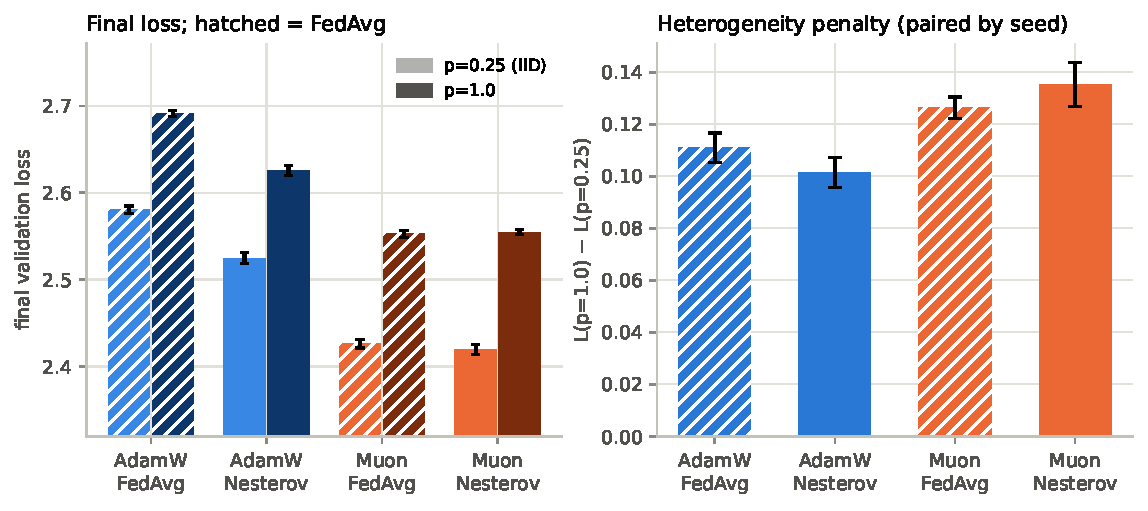
\includegraphics[width=0.95\linewidth]{fig5_e2_outer_momentum.pdf}
  \caption{H2. Left: final loss for each inner $\times$ outer combination at IID (lighter) and full skew (darker); hatched bars are FedAvg. Right: heterogeneity penalty $L(p{=}1) - L(p{=}0.25)$ paired by seed. Outer momentum slightly lowers the penalty for AdamW and slightly raises it for Muon.}
  \label{fig:h2}
\end{figure}

\Cref{fig:h2} and \cref{tab:h2} report the $2\times2$ ablation. Outer Nesterov momentum lowers AdamW's penalty by $R_{\mathrm{AdamW}} = 0.0095 \pm 0.0027$ (positive on all seeds) but gives Muon no rescue: $R_{\mathrm{Muon}} = -0.0088 \pm 0.0065$ (negative on all seeds). The per-seed differences $R_{\mathrm{Muon}} - R_{\mathrm{AdamW}}$ are $-0.027, -0.020, -0.009$.

\textbf{H2 is not supported; the predicted ordering is reversed.} At full skew, FedAvg-Muon ($2.5528$) and MuLoCo ($2.5548$) are statistically indistinguishable (per-seed differences $-0.007$, $-0.001$, $+0.003$). Even at IID, momentum helps Muon far less ($2.4264 \to 2.4196$) than AdamW ($2.5806 \to 2.5245$). Nesterov leaves a large residual penalty for both optimizers, as predicted. This pattern matches \citet{takezawa2026fedmuon}'s analysis that server momentum cannot remove the bias of LMO-based local
updates, though our experiment does not isolate that mechanism.

\begin{table}[t]
  \centering
  \caption{H2. Heterogeneity penalty (full skew minus IID, paired by seed) under each outer scheme, and the
  outer-momentum rescue $R_i$. H2 predicted $R_{\mathrm{Muon}} > R_{\mathrm{AdamW}} > 0$.}
  \label{tab:h2}
  \small
  \begin{tabular}{lccc}
    \toprule
    Inner optimizer & Penalty, FedAvg & Penalty, Nesterov & Rescue $R_i$ \\
    \midrule
    AdamW & $0.1110 \pm 0.0057$ & $0.1014 \pm 0.0059$ & $+0.0095 \pm 0.0027$ \\
    Muon  & $0.1264 \pm 0.0040$ & $0.1352 \pm 0.0086$ & $-0.0088 \pm 0.0065$ \\
    \bottomrule
  \end{tabular}
\end{table}

\subsection{Mechanism: parameter-space diagnostics disagree with the loss; function-space drift agrees}\label{sec:mechanism}

\begin{figure}[t]
  \centering
  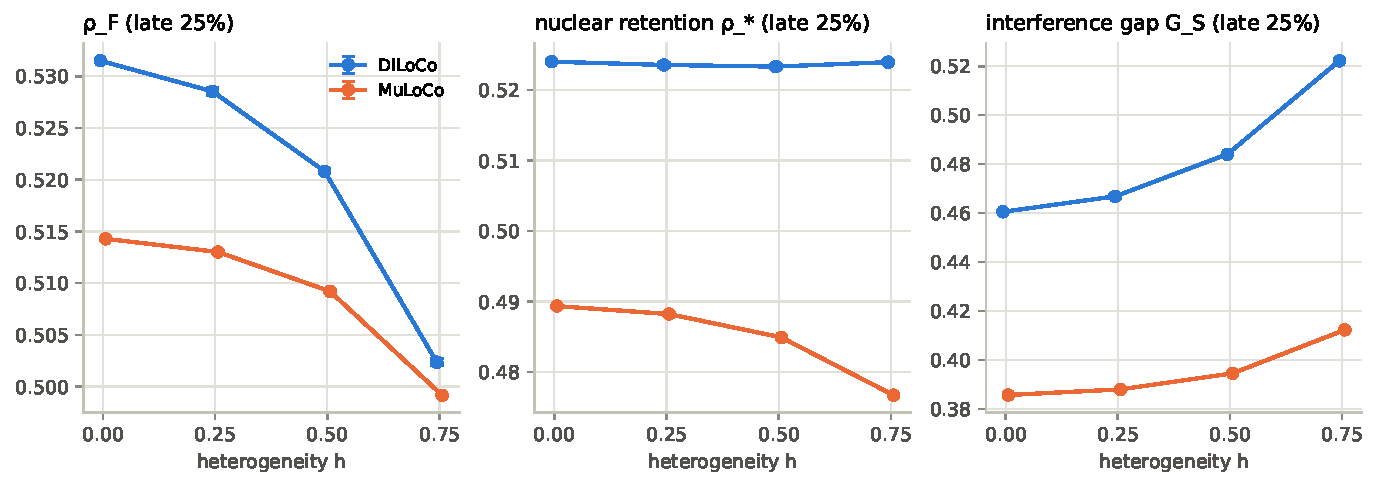
\includegraphics[width=\linewidth]{fig7_diagnostics_vs_h.pdf}
  \caption{Parameter-space diagnostics on the hidden matrices, averaged over the last 25\% of rounds (mean $\pm$ std over seeds; error bars are smaller than the markers). By these measures, MuLoCo's averaged updates lose less to
  cancellation than DiLoCo's and degrade less with heterogeneity, the opposite of their loss penalties.}
  \label{fig:diag}
\end{figure}

We planned to check H1's mechanism by asking whether the drift diagnostics fall more steeply with $h$ for whichever method degrades more. They do not (\cref{fig:diag}, \cref{tab:diag}). From IID to full skew, DiLoCo's norm retention falls from $0.532$ to $0.502$ and its interference gap rises from $0.461$ to $0.522$; MuLoCo's changes are about half as large ($0.514 \to 0.499$; $0.386 \to 0.412$). MuLoCo's averaged update is also better aligned with the outer momentum (${\approx}0.25$ vs.\ $0.05$-$0.09$) and with the data-parallel reference step ($0.383 \to 0.356$ vs.\ $0.312 \to 0.272$). Two further observations temper all of these measures: even at IID, $\rho_F$ is close to the orthogonal value $0.5$ and pairwise cosines are near zero late in training (\cref{fig:alignment}), so per-round pseudo-gradients are dominated by noise rather than by a shared direction; heterogeneity moves these quantities by only a few hundredths.

\begin{figure}[t]
  \centering
  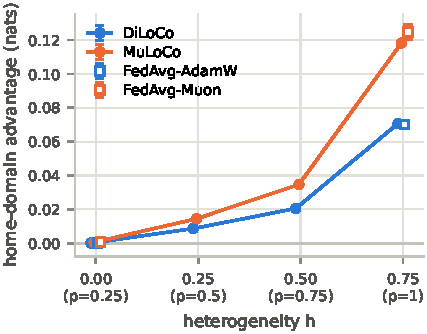
\includegraphics[width=0.55\linewidth]{fig9_home_advantage.pdf}
  \caption{Function-space drift (post-hoc). Home-domain advantage of the workers' local models just before averaging, at 75\% of training: for each domain, the mean loss of the other workers' local models minus the home worker's, averaged over domains. Filled markers: Nesterov outer; open squares: FedAvg (run at $p\in\{0.25,1\}$ only). Muon-based workers specialize ${\approx}1.7\times$ more within a 30-step round.}
  \label{fig:home}
\end{figure}

A different picture emerges in function space. Using the specialization matrices, we measure each worker's \emph{home-domain advantage}: how much better its local model is on its own domain than the other workers' local
models are, at the end of a round and before averaging. At IID, the advantage
is zero for all methods, as expected. At full skew it is $0.071 \pm 0.001$ for DiLoCo and $0.070 \pm 0.002$ for FedAvg-AdamW, but $0.118 \pm 0.001$ for MuLoCo and $0.125 \pm 0.004$ for FedAvg-Muon (\cref{fig:home}, \cref{tab:home}): within the same 30 steps, Muon workers move about $1.7\times$ further toward their home domain. This ordering (Muon-based above AdamW-based, outer optimizer nearly irrelevant) is exactly the ordering of the
heterogeneity penalties in \cref{tab:h2}.

% ======================================================================================================
\section{Discussion}\label{sec:discussion}

\paragraph{Why would better-aligned updates degrade more?} Our parameter-space diagnostics measure agreement among workers' updates and with a reference direction; they say little about how far each update moves the model's \emph{function}, or about where the averaged iterate settles. Muon's
step size is independent of gradient magnitude and it equalizes the singular values of each update, so directions with small gradient signal, plausibly the domain-specific ones, receive full-size steps. Over $H$ local steps on
skewed data this produces local models that are more specialized, which our home-domain measure detects directly. Averaging such models need not cancel much in parameter space (pseudo-gradients are near-orthogonal for every
method), yet the averaged model can still sit further from the global optimum, which is the fixed-point bias that \citet{takezawa2026fedmuon} analyze for LMO-based local updates and that momentum cannot remove. This account is consistent with all of our measurements but is not tested causally here.

\paragraph{Confounds we cannot rule out.} (i) MuLoCo's AdamW-managed parameters (embedding, output head, norms) use twice DiLoCo's inner learning rate ($1.5\times10^{-3}$ vs.\ $7.5\times10^{-4}$), as chosen by IID tuning, so part of the extra drift could come from these parameters rather than from Muon itself. (ii) Outer hyperparameters were tuned on IID data; a skew-tuned outer learning rate or momentum might recover some of MuLoCo's penalty. On IID data, MuLoCo's loss also varied less with outer momentum than DiLoCo's (range $0.048$ vs.\ $0.146$ nats over $\mu \in \{0, 0.3, 0.6, 0.9\}$ at $\eta_{\mathrm{out}}=0.8$), suggesting the outer step matters less for Muon even without skew. (iii) MuLoCo reaches lower loss, and absolute penalties at lower loss need not be directly comparable; the equalized $G_{\mathrm{DP}}$ at full skew is one way to read this.

\paragraph{Implications.} For practitioners, MuLoCo remains the better choice in absolute terms across the skews we tested, but its benefit should be expected to shrink as worker data diverge, and DiLoCo's outer momentum should not be relied on to protect it. Corrections that target drift directly (control variates~\cite{karimireddy2020scaffold}, the bias-corrected LMO of \citet{takezawa2026fedmuon}, or shorter $H$ for Muon workers) are the natural next step, and the home-domain advantage is a cheap signal for monitoring them.

% ======================================================================================================
\section{Limitations}\label{sec:limitations}
We study one model scale (51M parameters), one token budget (0.49B), $K=4$ workers, and one synchronization interval ($H=30$); drift is expected to grow with $H$, and the interaction with scale is unknown. Three seeds support
effect-size statements against a pre-stated rule, not formal significance tests. All hyperparameters were tuned on IID data, by design, to measure how a method tuned in the common setting degrades; this favors neither method a priori but means we do not report best-case non-IID performance. Weight decay is zero. Domains come from two sources and are unevenly distant (Wikipedia is much further from the others than the other three are from each other), so $h$ is not a perfect measure of how different workers' objectives are. The function-space analysis was designed after seeing the parameter-space results and uses three probe rounds. Workers are simulated sequentially, which is computationally equivalent to parallel execution but does not model stragglers or asynchrony.

% ======================================================================================================
\section{Conclusion}
Muon's advantage as DiLoCo's inner optimizer survives domain-heterogeneous data in absolute terms but erodes: its heterogeneity penalty is larger and grows faster with skew, consistent with federated-learning predictions about
client drift, and DiLoCo's outer momentum does not protect it. The parameter-space diagnostics used to explain MuLoCo's IID success point the wrong way under heterogeneity, while a simple function-space measure of worker specialization tracks the penalty. Low-communication training with Muon on heterogeneous data likely needs explicit drift correction.

\paragraph{Reproducibility.} All code, configurations, run manifests, per-run logs (\texttt{metrics.jsonl} with training loss every round, per-domain validation loss every 300 steps and all diagnostics), the scripts that produce
every figure and table in this paper (\texttt{analysis/plots.py}), and SHA-256 checksums of the 49 checkpoints are in the GitHub repository; the checkpoints are on Hugging Face. The processed data are rebuilt deterministically from pinned dataset revisions and verified by a content hash (\texttt{33c0c658fbf49a8a}).

\paragraph{Acknowledgments.} We thank the EECS 182 course staff at UC Berkeley, with special thanks to Professor Gireeja Ranade and PhD student
Mert Cemri for advising this project. Experiments were run on Modal's cloud GPU platform. We also thank the maintainers of the open datasets and software this work builds on: SlimPajama (Cerebras), the Wikimedia Foundation's
Wikipedia dumps, Hugging Face for dataset and model hosting, and PyTorch, including its \texttt{torch.optim.Muon} implementation. Use of AI assistants in this project is described in \cref{app:ai}.

\bibliographystyle{plainnat}
\bibliography{refs}

% ======================================================================================================
\clearpage
\appendix

\section{Hyperparameters}\label{app:hparams}
\begin{table}[!htbp]
  \centering
  \small
  \caption{Hyperparameters. Top: settings shared by every run. Bottom: the frozen per-method learning rates and outer-optimizer settings used in all production runs, chosen by IID tuning (\cref{app:tuning}).}
  \label{tab:hparams}
  \begin{tabular}{lp{0.66\linewidth}}
    \toprule
    Setting & Value \\
    \midrule
    Model & 8 layers, $d=512$, 8 heads (head dim 64), MLP $4\times$ GELU, RoPE, RMSNorm (pre-norm), QK-norm, no biases \\
    Parameters & 50.93M total; 25.17M non-embedding; 25.17M in Muon-managed matrices \\
    Vocabulary & GPT-2 (50{,}257, padded to 50{,}304), tied input/output embedding \\
    Sequence length / batch & 1{,}024 / 64 sequences (65{,}536 tokens) per step \\
    Steps / tokens & 7{,}500 / 491.5M \\
    Workers / sync interval & $K=4$, $H=30$ (250 rounds); 16 sequences per worker per step \\
    LR schedule & 250-step linear warmup, cosine decay to $0.1\times$ peak (indexed by inner step) \\
    AdamW & $\beta=(0.9, 0.95)$, $\epsilon=10^{-8}$, weight decay 0 \\
    Muon & Nesterov momentum 0.95, 5 Newton--Schulz steps, AdamW-matched RMS scaling, weight decay 0 \\
    Gradient clipping & global norm 1.0, per worker per step \\
    Precision & bf16 autocast; fp32 weights, optimizer and outer state \\
    \midrule
    DP-AdamW & lr $1.5\times10^{-3}$ \\
    DP-Muon & Muon lr $1.2\times10^{-2}$; AdamW lr $1.5\times10^{-3}$ (embedding, head, norms) \\
    DiLoCo & inner lr $7.5\times10^{-4}$; outer lr 0.8, Nesterov momentum 0.6 \\
    MuLoCo & Muon lr $1.2\times10^{-2}$, AdamW lr $1.5\times10^{-3}$; outer lr 0.8, momentum 0.6 \\
    FedAvg-AdamW / FedAvg-Muon & inner lrs as DiLoCo / MuLoCo; outer lr 1, momentum 0 \\
    \bottomrule
  \end{tabular}
\end{table}

\section{Tuning results}\label{app:tuning}
All tuning runs use seed 0 and IID data. Stage A runs are full length; Stages B and C use half-length runs (3{,}750 steps with the schedule compressed), so their losses are higher than full-length losses.

\begin{table}[!htbp]
  \centering
  \small
  \caption{Tuning results (seed 0, IID data; final balanced validation loss). Stage A runs are full length; Stages B and C are half length (3{,}750 steps, schedule compressed), so their losses are higher and comparable only with each other. Bold marks the selected setting; Stage C's $\times1$ entries are the matching Stage B runs.}
  \label{tab:tuning}
  \begin{tabular}{lcccccc}
    \toprule
    \multicolumn{7}{l}{\emph{Stage A: DP learning rate (full length), final balanced loss}} \\
    AdamW lr & $7.5\times10^{-4}$ & $\mathbf{1.5\times10^{-3}}$ & $3\times10^{-3}$ & $6\times10^{-3}$ & & \\
     & 2.3302 & \textbf{2.3079} & 2.3241 & 2.3447 & & \\
    Muon lr & $1.5\times10^{-3}$ & $3\times10^{-3}$ & $6\times10^{-3}$ & $\mathbf{1.2\times10^{-2}}$ & $2.4\times10^{-2}$ & \\
     & 2.2523 & 2.2557 & 2.2536 & \textbf{2.2490} & 2.2516 & \\
    \midrule
    \multicolumn{7}{l}{\emph{Stage B: outer $(\eta_{\mathrm{out}}, \mu)$ (half length)}} \\
    $(\eta_{\mathrm{out}}, \mu)$ & (0.5, 0.6) & (0.5, 0.9) & (0.8, 0) & (0.8, 0.3) & \textbf{(0.8, 0.6)} & (0.8, 0.9) \\
    DiLoCo & 2.7524 & 2.8582 & 2.7955 & 2.7383 & \textbf{2.7335} & 2.8790 \\
    MuLoCo & 2.5322 & 2.5614 & 2.5638 & 2.5312 & \textbf{2.5157} & 2.5632 \\
    $(\eta_{\mathrm{out}}, \mu)$ & (1.0, 0.6) & (1.0, 0.9) & & & & \\
    DiLoCo & 2.7384 & 2.9201 & & & & \\
    MuLoCo & 2.5205 & 2.5684 & & & & \\
    \midrule
    \multicolumn{7}{l}{\emph{Stage C: inner lr multiplier at outer (0.8, 0.6) (half length)}} \\
    multiplier & $\times0.25$ & $\times0.5$ & $\times1$ & $\times2$ & & \\
    DiLoCo (AdamW lr) & 2.7499 & \textbf{2.6867} & 2.7335 & 2.7900 & & \\
    MuLoCo (Muon lr) & -- & 2.5150 & \textbf{2.5157} & 2.5135 & & \\
    \bottomrule
  \end{tabular}
\end{table}
MuLoCo's three Stage C values differ by less than seed noise, so its Muon rate was kept at the Stage A value. DiLoCo's
outer setting was chosen before its inner rate was halved and was not re-swept.

\section{Additional results}\label{app:figures}

\begin{table}[!htbp]
  \centering
  \caption{Late-training diagnostics (mean over the last 25\% of rounds, then over 3 seeds; all across-seed stds
  $\le 0.003$). ref.\ cos is the mean over the three probe rounds.}
  \label{tab:diag}
  \small
  \begin{tabular}{llcccccc}
    \toprule
    Method & $p$ & $\rho_F$ & pair cos & mom.\ align & $\rho_*$ & interf.\ gap & ref.\ cos \\
    \midrule
    DiLoCo & 0.25 & 0.532 & 0.044 & 0.047 & 0.524 & 0.461 & 0.312 \\
           & 0.5  & 0.529 & 0.039 & 0.052 & 0.524 & 0.467 & 0.309 \\
           & 0.75 & 0.521 & 0.028 & 0.064 & 0.523 & 0.484 & 0.297 \\
           & 1.0  & 0.502 & 0.003 & 0.086 & 0.524 & 0.522 & 0.272 \\
    MuLoCo & 0.25 & 0.514 & 0.019 & 0.247 & 0.489 & 0.386 & 0.383 \\
           & 0.5  & 0.513 & 0.018 & 0.249 & 0.488 & 0.388 & 0.380 \\
           & 0.75 & 0.509 & 0.012 & 0.253 & 0.485 & 0.395 & 0.374 \\
           & 1.0  & 0.499 & $-0.001$ & 0.266 & 0.477 & 0.412 & 0.356 \\
    FedAvg-AdamW & 0.25 & 0.519 & 0.027 & -- & 0.516 & 0.477 & 0.267 \\
                 & 1.0  & 0.495 & $-0.007$ & -- & 0.518 & 0.530 & 0.235 \\
    FedAvg-Muon  & 0.25 & 0.508 & 0.011 & -- & 0.484 & 0.395 & 0.367 \\
                 & 1.0  & 0.496 & $-0.005$ & -- & 0.474 & 0.416 & 0.341 \\
    \bottomrule
  \end{tabular}
\end{table}

\begin{table}[!htbp]
  \centering
  \caption{Home-domain advantage of local models before averaging at 75\% of training (nats; mean $\pm$ std over 3
  seeds). Post-hoc analysis.}
  \label{tab:home}
  \small
  \begin{tabular}{lcccc}
    \toprule
    Method & $p=0.25$ & $p=0.5$ & $p=0.75$ & $p=1$ \\
    \midrule
    DiLoCo       & $0.000 \pm 0.001$ & $0.009 \pm 0.000$ & $0.021 \pm 0.002$ & $0.071 \pm 0.001$ \\
    MuLoCo       & $0.001 \pm 0.001$ & $0.014 \pm 0.000$ & $0.035 \pm 0.001$ & $0.118 \pm 0.001$ \\
    FedAvg-AdamW & $0.000 \pm 0.001$ & -- & -- & $0.070 \pm 0.002$ \\
    FedAvg-Muon  & $0.001 \pm 0.001$ & -- & -- & $0.125 \pm 0.004$ \\
    \bottomrule
  \end{tabular}
\end{table}

\begin{figure}[!htbp]
  \centering
  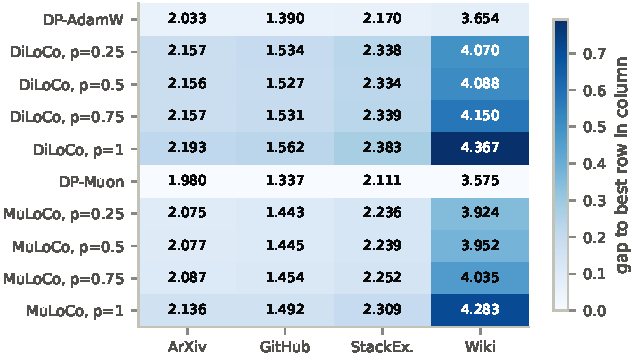
\includegraphics[width=0.75\linewidth]{fig4_domain_heatmap.pdf}
  \caption{Final per-domain validation loss (mean over seeds). Colour encodes the gap to the best row in each domain.
  Most of the heterogeneity penalty is on Wikipedia.}
  \label{fig:heatmap}
\end{figure}

\begin{figure}[!htbp]
  \centering
  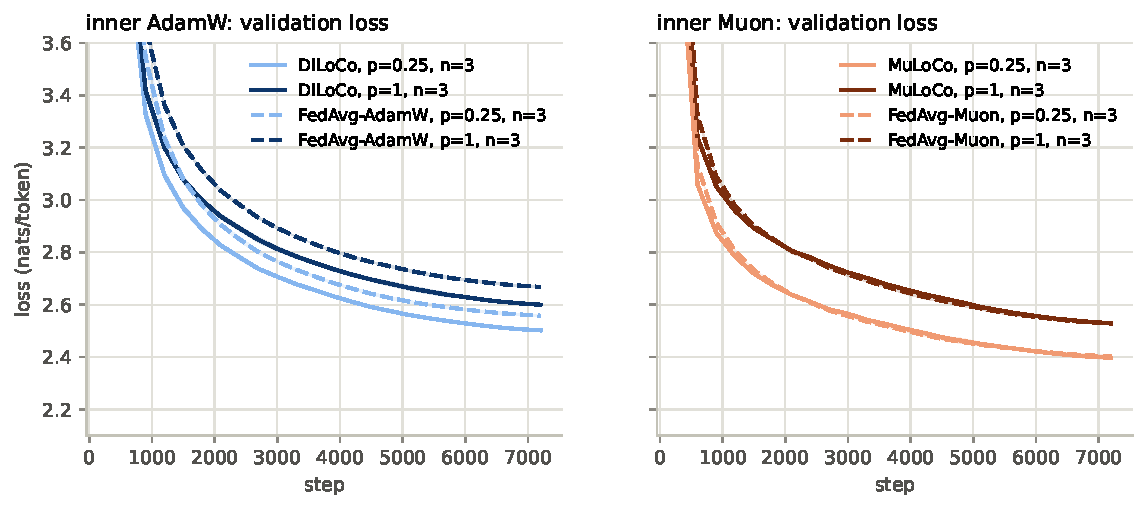
\includegraphics[width=\linewidth]{fig1b_loss_curves_e2.pdf}
  \caption{Validation loss curves for the outer-optimizer ablation: Nesterov (solid) vs.\ FedAvg (dashed) at IID
  (light) and full skew (dark), per inner optimizer. Bands are $\pm1$ std over 3 seeds.}
  \label{fig:curves_e2}
\end{figure}

\begin{figure}[!htbp]
  \centering
  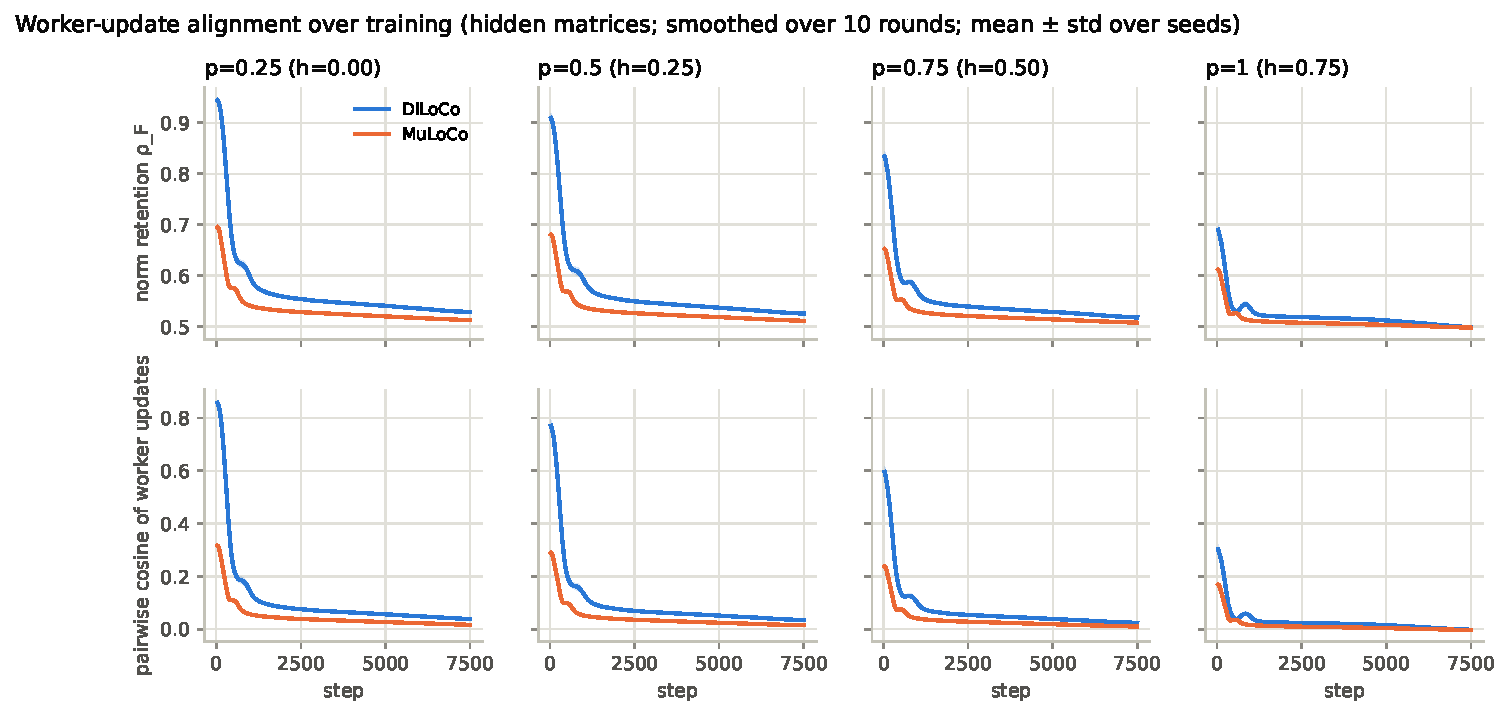
\includegraphics[width=\linewidth]{fig6_alignment_over_training.pdf}
  \caption{Norm retention $\rho_F$ and mean pairwise cosine of worker pseudo-gradients over training, per skew level.
  After the first ${\sim}1{,}000$ steps both methods approach the orthogonal-worker values ($\rho_F \approx 0.5$,
  cosine $\approx 0$) at every skew.}
  \label{fig:alignment}
\end{figure}

\begin{figure}[!htbp]
  \centering
  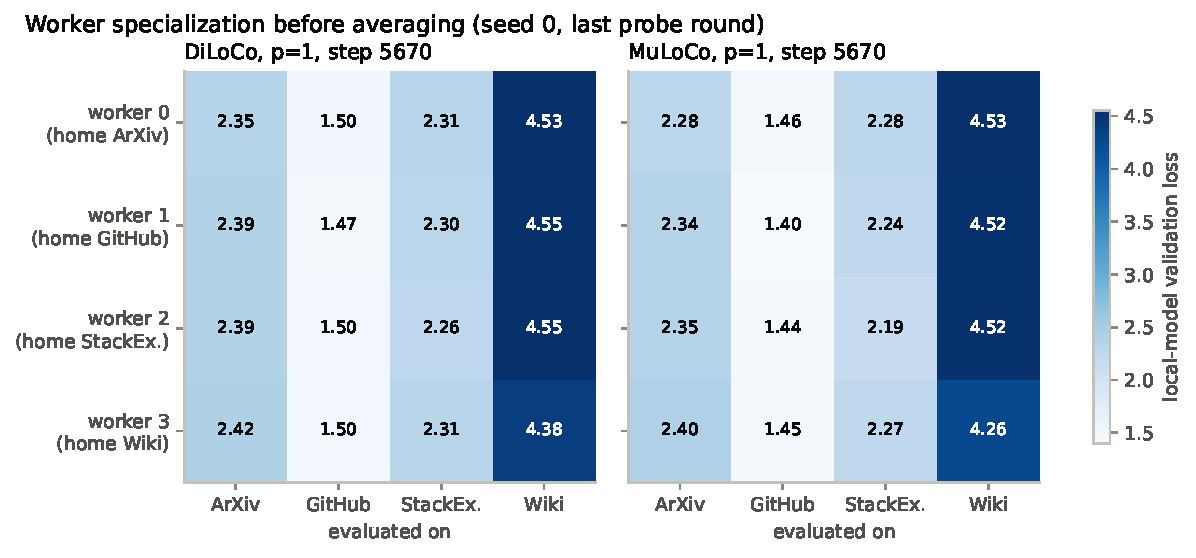
\includegraphics[width=\linewidth]{fig8_specialization.pdf}
  \caption{Specialization matrices at full skew (seed 0, 75\% of training): each worker's local model, just before
  averaging, evaluated on each domain. Diagonal entries (home domains) are lower; the effect is larger for MuLoCo.}
  \label{fig:specialization}
\end{figure}

\clearpage
\section{Use of AI tools}\label{app:ai}
We used Anthropic's Claude (via Claude Code) as an assistant throughout this project. It helped implement the training, data-processing, and analysis code; refine the experimental design and tuning protocol; launch and monitor training runs on Modal and back up their results; produce the figures and tables; and draft parts of this report. The research question and hypotheses come from our original project proposal, and all experimental decisions (scope, tuning stages, budget, and which runs to launch) were made by the authors. We reviewed the code, verified results against the logged
run data, and edited the text, and we take full responsibility for the content of this paper.

\end{document}